\section{Sensoren}
\label{sec:sensor}

Zur Detektion von Kot oder Urin steht eine Vielzahl an Sensoren zur
Verfügung. Eine Auswahl derer wären: Gas, Temperatur, Feuchtigkeit,
Gewicht, Luftfeuchtigkeit, uvm. Die Auswahl verringert sich durch
einige ergonomische und medizinische und technische Anforderungen, wie
zum Beispiel Hautverträglichkeit, Wasserfestigkeit, Langlebigkeit,
Größe und Waschbarkeit. Durch diese Spezifikationen fielen zum
Beispiel Gas, Luftfeuchtigkeit aus der Auswahl, da Diese nicht
wasserfest sind und somit nicht in der Windel zum Einsatz kommen
können. Ein Gewichts- bzw Drucksensor  konnte nicht verwendet werden,
da das Aufsetzen/Hinsetzen des Babys zum Auslösen führen würde.
Nach Ausschluss vieler möglicher Detektionsverfahren, wurde in diesem
Projekt das Hauptziel auf die Konstruktion und den Entwurf eines
Feuchtigkeitssensors, welcher in Zusammenarbeit mit einem
Temperatursensor die Ausscheidung eines Babys erkennt und in Folge
dessen ein Signal versendet, wie es im Kapitel „Kommunikation“ näher
beschrieben wird gelegt. Um ein Fehlauslösen und somit einen Fehlalarm
zu vermeiden, wurden die Sensoren miteinander verknüpft und nur ein
Auslösen Beider führt zur Sendung eines Trigger Signals.
Im Folgenden werden die verwendeten Sensoren, sowie deren
Funktionsweise näher erläutert.


\subsection{Temperatursensor}
Da die Ausscheidungen eines Menschen die Körperkerntemperatur besitzen
und diese um einige Grad höher ist als die Oberflächentemperatur, kann
dieser Unterschied leicht detektiert werden und als Signal verwendet
werden. Die anfängliche Idee eine Temperaturschwelle festzulegen und
bei Überschreitung Dieser ein Signal auszulösen, wurde verworfen da
das Ansteigen der Umgebungstemperatur oder ein Fieber zum Anschlagen
des Sensors führen würde und somit einen Fehlalarm auslösen könnte.
Diese Änderungen entstehen über einen längeren Zeitraum, wohingegen
das Ausscheiden von Exkrementen in kurzer Zeit stattfindet. Die daraus
resultierende schnelle Veränderung lässt sich einfach detektieren und
deutet mit sehr hoher Wahrscheinlichkeit auf Exkretion hin.
Die erste Version des Sensors wurde mittels einer Wheatstone-Brücke
realisiert. Diese Schaltung ist eine Widerstandsbrücke, welche aus
zwei parallelgeschalteten Spannungsteilern mit identischen
Widerständen besteht. Mindestens einer dieser Widerstände wird als PTC
oder NTC realisiert. Bei einer abgeglichenen Brückenschaltung ist das
Potenzial zwischen den Mittelpunkten der Spannungsteiler Null. Sobald
sich also ein Widerstand ändert, ändert sich auch der
Potenzialunterschied. Ein großer Vorteil dieser Messbrücke ist die
Genauigkeit der Messung, welche ohne Offset vorliegt. Jedoch ist
dieser Vorteil in diesem Projekt ein großer Nachteil, da die Schaltung
sehr sensibel ist. Außerdem ist das Abgleichen quasi unmöglich durch
die unterschiedlichen Körpertemperaturen bzw. Außentemperaturen. 
Aufgrund dieses Nachteils und der nicht vorhandenen Notwendigkeit der
Genauigkeit, wurde sich gegen eine Wheatstone-Brücke entschieden.

\begin{figure}
\centering
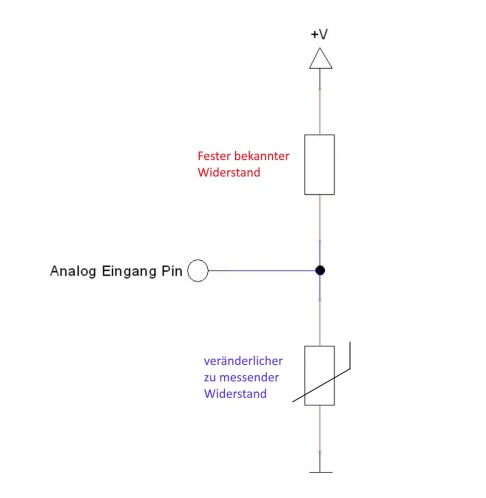
\includegraphics[width=.6\textwidth]{includes/sensor_pics/486px-KY-013_VoltDivide.jpg}
\caption{Aufbau der Sensorschaltung}
\label{fig:tempsens}
\end{figure}

Die zweite Version des Sensors wurde mittels eines analogen
Temperatursensors (KY-013) realisiert, welcher im Arduino Sensor kit
vorhanden ist. Dieses Modul besteht aus einem festen Widerstand als
Referenz und zur Strombegrenzung in Reihe mit einem
temperaturveränderlichen NTC-Thermistor (Bild \ref{fig:tempsens}),
welcher mit steigender Temperatur einen geringer werdenden Widerstand
hat (Bild \ref{fig:tempkurve}).

\begin{figure}
\centering
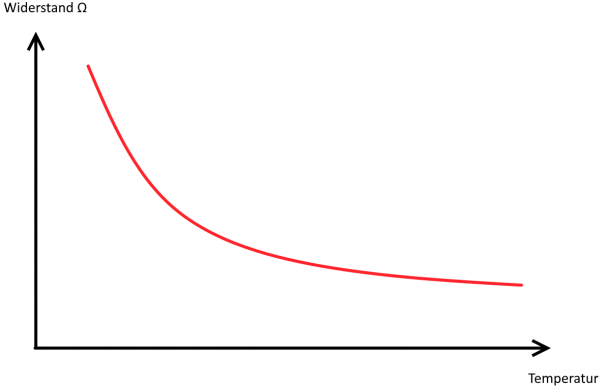
\includegraphics[width=.6\textwidth]{includes/sensor_pics/610px-KY-013_NTC-Kurve.png}
\caption{Änderung des Widerstands mit steigender
Temperatur.}
\label{fig:tempkurve}
\end{figure}

``Diese Änderung des Widerstands lässt sich mathematisch annähern und
in einen linearen Verlauf umrechnen und den Temperaturkoeffizienten
(Abhängigkeit von Widerstandsänderung zur Temperaturänderung)
bestimmen. Mittels diesen lässt sich somit dann immer die aktuelle
Temperatur errechnen, wenn man den aktuellen Widerstand kennt. Dieser
Widerstand lässt sich mit Hilfe eines Spannungsteilers bestimmen, wo
sich eine bekannte Spannung über den bekannten und den unbekannten
(veränderlichen) Widerstand aufteilt. Mittels dieser gemessenen
Spannung lässt sich dann der Widerstand berechnen - die genaue
Berechnung ist in dem unten stehenden Codezeilen
enthalten.''\footnote{Text und Bilder entnommen von:
\url{http://sensorkit.joy-it.net/index.php?title=KY-013_Temperatur-Sensor_Modul}.}

\begin{lstlisting}[language=C, caption=Umrechnung des Analogwerts in Temperatur.]
/* Calculate Temperature from incomming Values */
double Thermistor(int RawADC) {
   double Temp;
   Temp = log(10000.0 * ((1024.0/RawADC - 1)));
   Temp = 1/(0.001129148 + (0.000234125 + (0.0000000876741*Temp*Temp))*Temp);
   Temp = Temp - 273.15;            // Convert Kelvin to Celcius
   //Temp = (Temp * 9.0)/ 5.0 + 32.0; // Convert Celcius to Fahrenheit
   return Temp;
}
\end{lstlisting}

\begin{lstlisting}[language=C, caption=Trigger für Exkretion durch
Temperaturvergleich.]
bool tempSensor (){
   bool returnValueTemp = false;
    
   int readVal = analogRead(sensorPinTemp);
   double temp =  Thermistor(readVal);
	
   difftemp = readVal - oldtemp;
   if (oldtemp != 0 && difftemp > 30) {
      returnValueTemp = true;
   }
   oldtemp = readVal;
   //Serial.println(temp);  // display tempature
   //Serial.println(readVal);  // display tempature
			  
   return returnValueTemp;
}
\end{lstlisting}

Wie im Code zu sehen ist, wurde er so umgeschrieben, dass er auf eine
schnelle Änderung der Temperatur anspricht, was wie oben beschrieben
auf Exkretion hindeutet\footnote{Der komplette Code ist auf
\url{https://github.com/jomaway/poop-face-detection_sensor}.}.
Im Gegensatz zum Feuchtigkeitssensor, welcher flächendeckend in die
Einlage eingenäht ist, misst der Temperatursensor sehr punktuell. Dies
stellt ein Problem dar, da je nach Geschlecht des Babys der Urin an
einer anderen Stelle ausgeschieden wird. Bei Mädchen eher zentral und
bei Jungen etwas weiter nach vorne versetzt. Eine Lösung wäre es, zwei
verschiedene, geschlechtsspezifische Modelle der Einlage anzufertigen.
Eine andere Lösung wäre es, zwei Sensoren zu verwenden, um an beiden
Stellen detektieren zu können, was aber die Kosten des Produkts
steigern würde. Ein nicht praktikabler Lösungsweg wäre eine mittige
Anbringung des Sensors. Die Flüssigkeit würde sich zwar im Stoff bis
dorthin ausbreiten, jedoch wäre die Temperatur bis dort so weit
abgekühlt, dass eine sichere Detektion nicht mehr sichergestellt
werden kann.
Das verwendete Modul ist durch seine rechteckige Form nur für einen
Prototype geeignet. Für die weitere Entwicklung bzw. Verwendung des
Poop-Face-Detection Systems würde ein anderer Sensor, wie ein TMP36
oder Ähnliche mehr Sinn machen, da die Form wesentlich ergonomischer
ist und dieser auch einfach anzuschließen und anzusteuern ist.

\subsection{Kapazitiver Feuchtigkeitssensor}
\label{sec:cap_sensor}

Dieses Kapitel befasst sich mit den Anforderungen und der Funktionsweise eines kapazitiven Feuchtigkeitssensors. Zudem wird der Unterschied und die Vor- und Nachteile eines kapazitiven zu einem resistiven Feuchtigkeitssensor dargestellt. Gegen Ende soll noch die praktische Entwicklung und die Probleme des Sensors beschrieben werden.


\subsubsection{Anforderungen}
\label{sec:cap_requirements}
Um die Feuchtigkeit in der Windel zu detektieren wird neben dem Wärmesensor ein kapazitiver Feuchtigkeitssensor verwendet. Der Feuchtigkeitssensor muss unter anderem medizinsch unbedenklich sein, da er direkt in der Windel integriert ist. Weil der Sensor in Windeln aus Baumwolle, die wiederverwendet und gewaschen werden, zum Einsatz kommt, soll der Sensor zusätzlich robust sein und eine lange Lebensdauer besitzen, und dabei nichts von seiner Funktion einbüßen.

\begin{description}
\item[Medizinische Unbedenklichkeit:]
Die medizinsche Unbedenklichkeit umfasst im wesentlichen zwei Kernpunkte. Einerseits dürfen keine zu starken Ströme fließen, anderseits darf der Sensor nicht korrodieren. Da der Sensor im wesentlichen aus zwei in Reihe geschalteten Kondesatoren besteht (siehe Kapitel "Funktionsweise") gibt es hohe Einschaltströme, da in der Kondesator im entladenen Zustand beim Einschaltvorgang einen unendlich kleinen Widerstand besitzt. Dieser Einschaltstrom lässt sich mit einem in Reihe geschaltetem Widerstand begrenzten. Diese Begrenzung ist wichtig da der Körper einen Innenwiderstand von 1kOhm\footnote{https://www.arbeitsschutz-schulen-nds.de/fachbezogene-themen/technik-werken/gefaehrdungen/durch-elektrische-energie/der-menschliche-koerper-als-widerstand/} besitzt. So können gravierende Zellschäden vermieden werden. 
Korrosion von Metallen ist ein weiteres großes Problem. Korrodiert der Sensor in der Windel werden unter anderem Metallatome und Metallradikale freigesetzt, die für den Körper des Kindes bedenklich sein können. Der leitende Faden wird aus Stahl gefertigt, ein Material das größtenteils aus Eisen, Chrom und Nickel besteht. Untersuchungen bestätigen das die Langzeitauswirkungen von Metallionen, z.B. durch Aufnahme über die Schleimhäute in Darm oder Vagina, zu "immunologischen und toxischen Reaktionen"\footnote{http://www.deguz.de/fachkreise/fachinformationen/metalle-und-Metallischer-zahnersatz/toxische-effekte-von-metallen-im-organismus.html} führen kann. Dadurch wird dann z.B. die "Ausschüttung von entzündungsfördernd wirkenden Botenstoffen" und "die Bildung freier Radikale" gefördert.
	
 \item[Lebensdauer und Robustheit:]
Eine wichtige Anforderung an den Sensor ist eine lange Lebensdauer. Der Sensor soll in die Stoffwindel integriert werden und muss daher ständiger Feuchtigkeit und auch dem Waschen in der Waschmaschine standhalten. Damit einhergehend darf der Sensor nicht korridieren und damit Metallradikale abgeben (siehe Abschnitt "Medizinische Unbedenklichkeit"). Die lange Lebensdauer soll durch zwei physikalische Charaktersitika erreicht werden. Da der Sensor kapazitiv wirken soll, fließt kein Strom zwischen den beiden Fäden, die als Kondensator wirken. Daher findet kein Ladungsaustausch statt und die Fäden korridieren im Idealfall nicht. Da aber Stoff auch leitend ist, kann man einen kleinen Stromfluss nicht verhindern. Das zweite Charakteristikum, neben der Isolation der zwei Metallfäden, ist die Flexibiltät der Metallfäden. Die darf auch nach mehrmaligem Waschen (Aufwärmung und Abkühlung) nicht abnehmen und der Draht nicht versteifen. Dadurch würde er leicht brechen und die Messungen werden nicht mehr möglich. 

 \item[Verlässlichkeit:]
Mit der langen Lebensdauer von Baumwollwindeln muss auch garantiert werden, dass der integrierte Sensor so lange funktioniert. Funktioniert dieser innerhalb der Lebensdauer von Stoffwindeln nicht mehr muss dieser ausgetauscht werden. Das ist aufwändig und will somit vermieden werden. Zudem darf sich die Kapazität des Sensors nicht gravierend ändern, da sonst die programmtechnischen Grenzen falsch gesetzt sind und der Kapazititätsanstieg durch Feuchtigkeit nicht mehr garantiert ist. Im besten Fall verhindert man eine Alterung und Korrosion der Metallfäden in der Windel.  
\end{description}

\subsubsection{Funktionsweise}
Die Detektion von Feuchtigkeit in der Windel gelingt mit einem kapazitiven Feuchtigkeitsmesser.

%Bild kapazitver Feuchtigkeitssensor
\begin{figure}[ht]
	\centering
		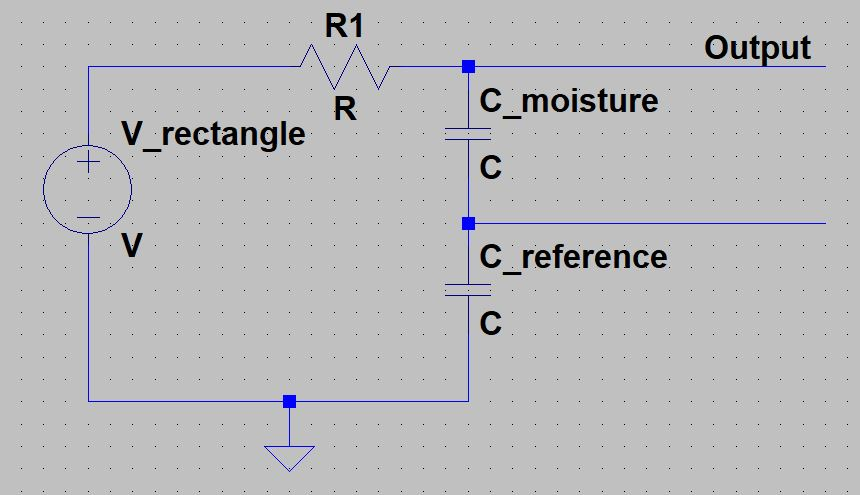
\includegraphics[width=0.6\textwidth]{includes/kom/graphics/cap_sensor_circuit}
	\caption{Prinzipschaltung kapazitiver Sensor}
	\label{fig:cap_sensor}
\end{figure}

Wie in der Grafik dargestellt werden zwei Kondensatoren und ein Widerstand in Reihe geschalten und die Spannung über einem Kondensator abgenommen. Da der Arduino Rechteckspannung erzeugen kann wirken die Kondesatoren wie Widerstände. Erhöht man nun die Kapazität des einen Sensors ändert sich der jeweilig anteilige Spannungsabfall.

Mit dem Arduino lässt sich die Spannung auslesen und nach geeigneter Kalibierung ein Grenzwert finden. Wird ein signifikanter Einbruch der Ausgangsspannung detektiert wird im Arduino die entsprechende Variable gesetzt wird per BLE ein entsprechendes Signal an den aufnehmenden Raspberry Pi geschickt.

 
\subsubsection{Unterschiede und Vor-/ Nacheile zum resistiven Feuchtkeitssensor}
Nachdem der prinzipielle Aufbau und die Funktionsweise muss man noch auf den wesentlichen Unterschied zum resistiven Feuchtigkeitssensor erwähnen. Wie vom Namen ableitbar erkennt der resitive Widerstandssensor Feuchtigkeit über eine Widerstandsmessung. Ist die Windel bzw. das allgemeine Umfeld trocken ist der Widerstand groß und es fließt kaum Strom. Wird das Umfeld nun leitbar gemacht, etwa durch Urin oder Wasser, steigt die Leitfähigkeit es kann durch einen Mikrokontroller eine Widerstandsänderung ausgelesen werden. 

Vorteile des restiven Feuchtigkeitsensors  ist die leichte Installation in die Windel. Mit Hilfe des Arduinos lässt sich recht einfach der Spannungsabfall und der daraus resultierende Stromfluss auslesen. D.h. mit relativ wenig Aufwand bekommt man schon auswertbare Ergebnisse. Das ist wiederum ein Nachteil des kapazitiven Feuchtigkeitssensors. Uns hat es einigen Aufwand gekostet die Simulation, Messungen und Berechnungen soweit in Einklang zu bringen das wir ein auswertbares Signal und einen geeigneten Triggerpunkt gefunden hatten mit dem man die Feuchtigkeit auslesen kann.

Im Gegensatz dazu ist der große Vorteil des kapaztiven Feuchtigkeitssensor zum resistiven die nicht einsetzende Korrosion. Da nicht mit Stromflüssen gearbeitet wird, sondern mit Kapazitätsunterschieden, korridieren die Metalldrähte nicht und man bekommt eine signifikant längere Lebensdauer der Drähte in der Windel.  

\subsubsection{Umsetzung und Entwicklung in der Praxis}
Angefangen mit der Konzeption haben wir mit LT-Spice-Simulationen. Dafür mussten wir herausfinden wie groß die Kapazität der zwei parallelen Drahtfäden in der Windel ist. Nach den Anfangs sehr kleinen und detektierbaren Kapazitäten mit einer einfachen parallelen Form wurde schnell umgedacht und durch Biegung der Drahtfäden die Länge der Leiterbahnen vergrößert. 

%Bild vom finalen Konzept
\begin{figure}[ht]
	\centering
		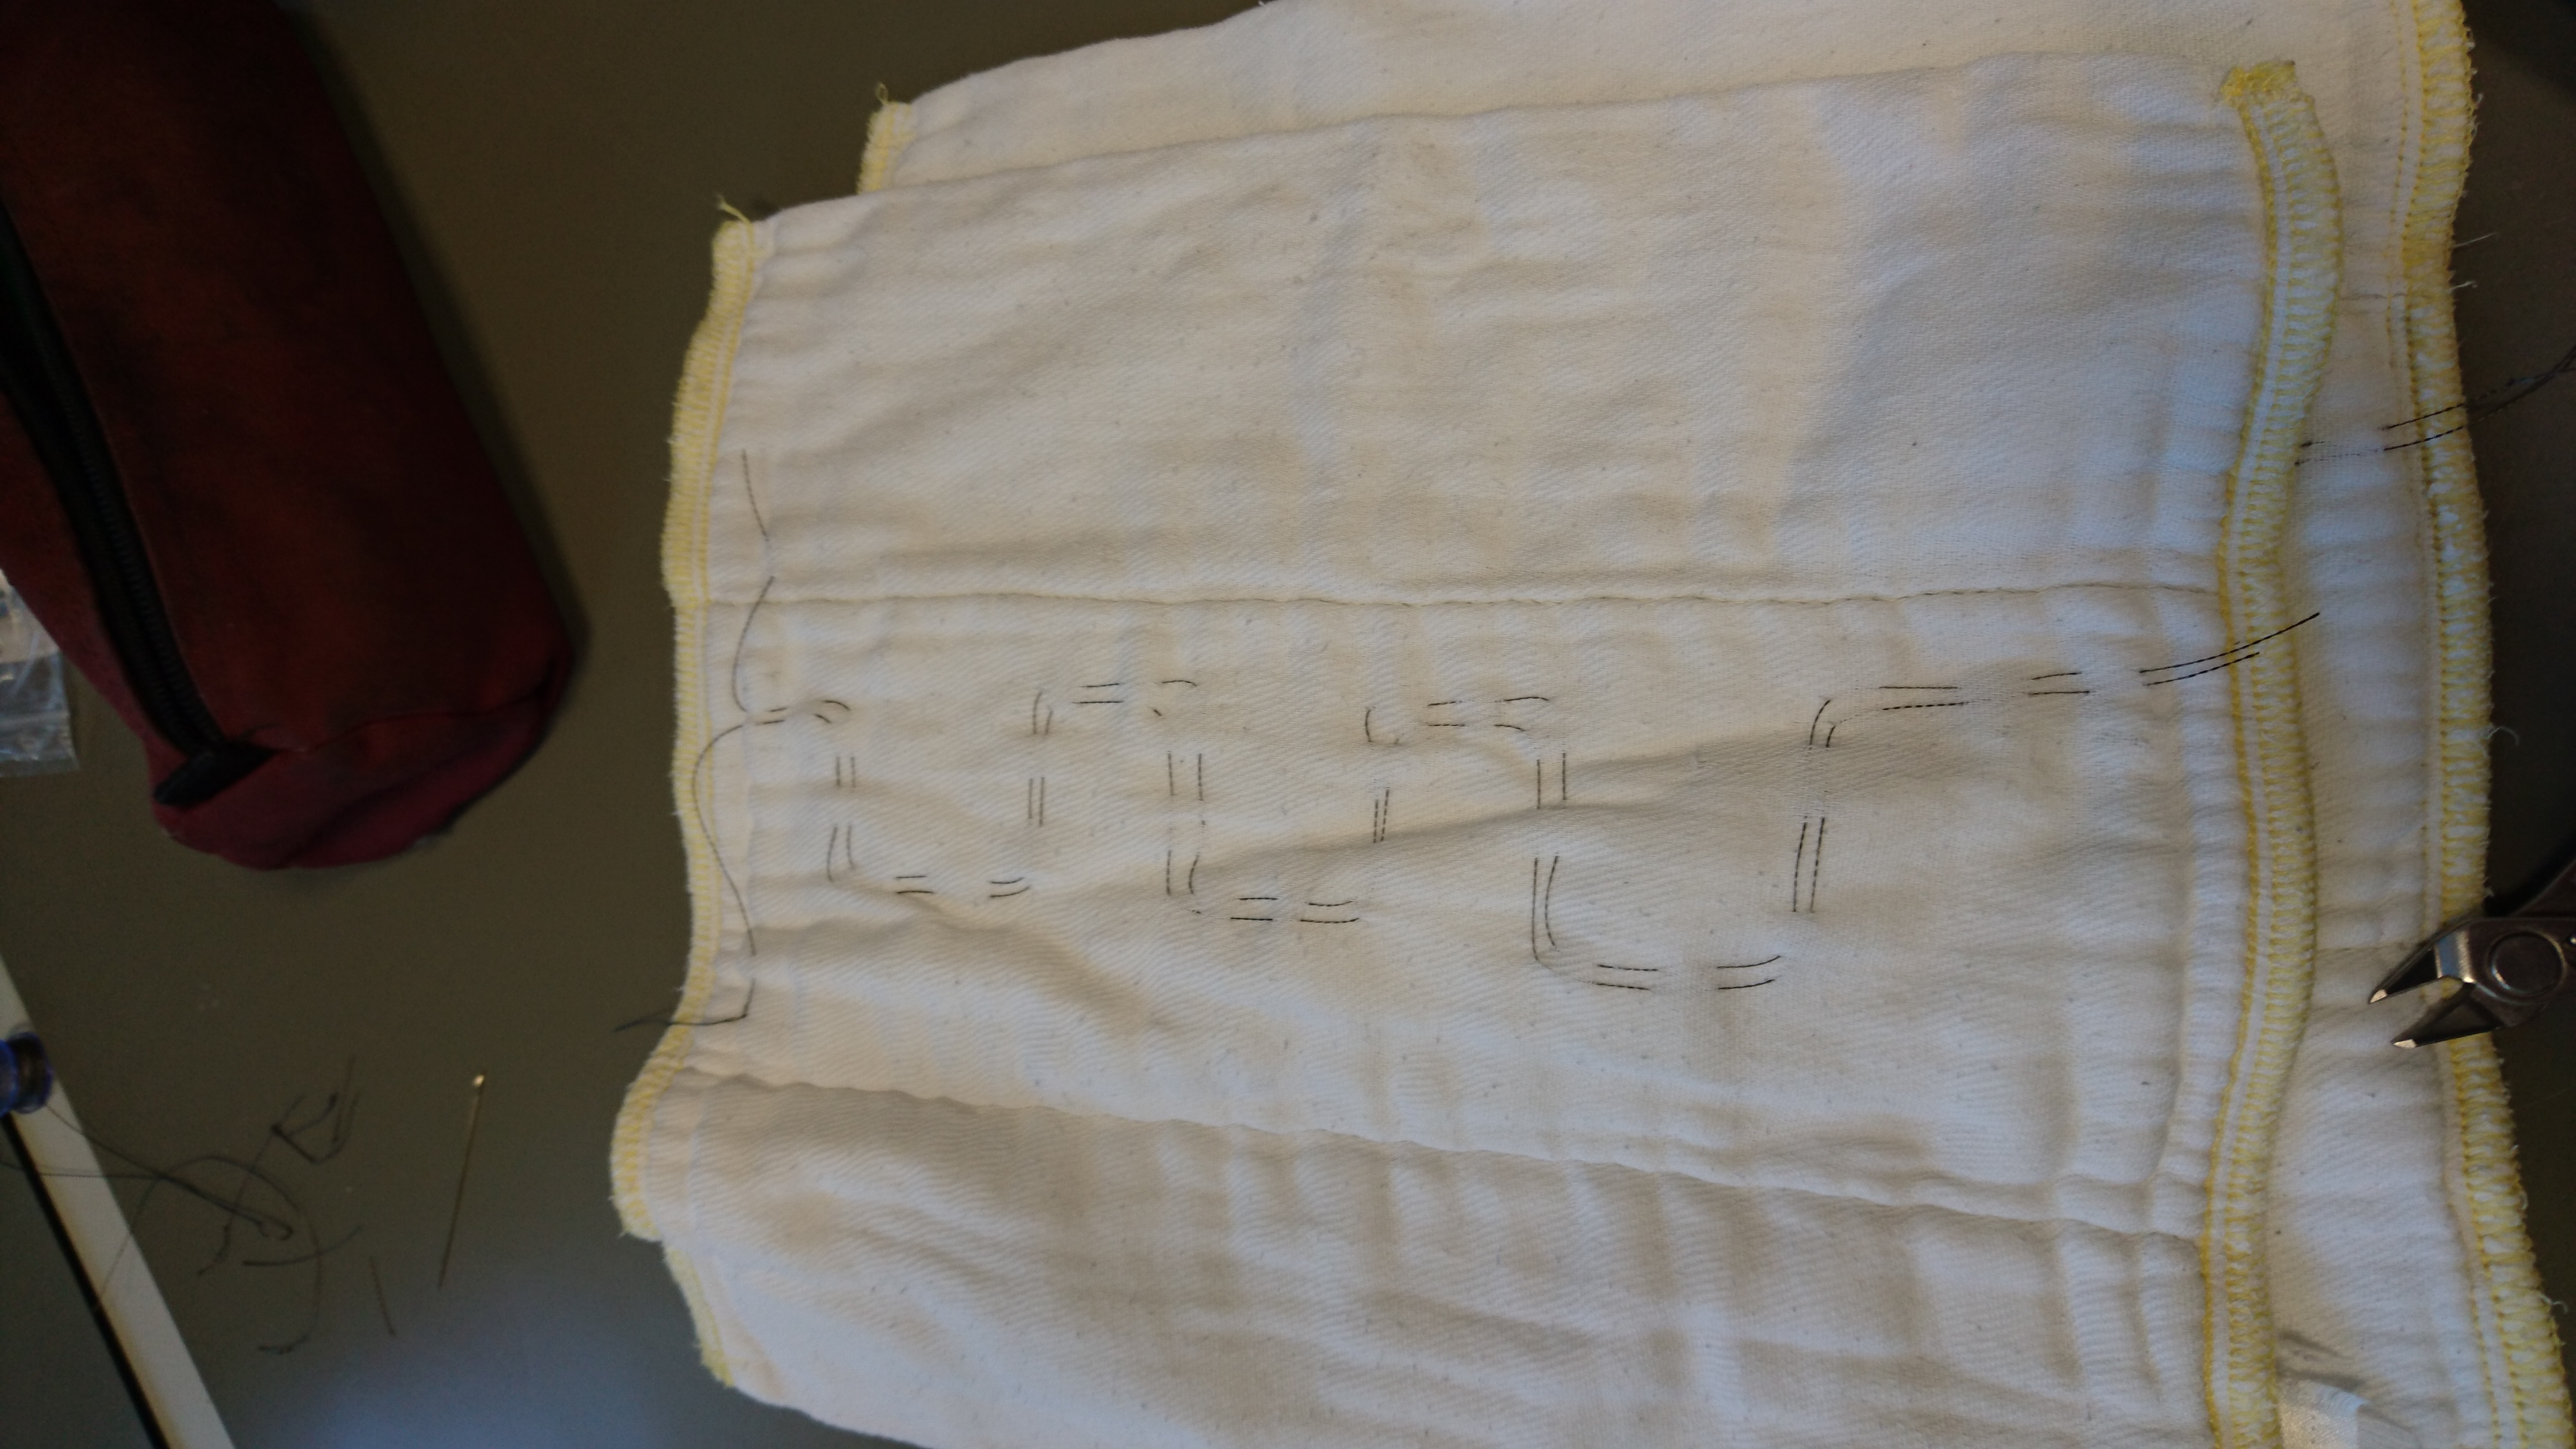
\includegraphics[width=0.6\textwidth]{includes/kom/graphics/cap_sensor_final}
	\caption{Finales Konzept Feuchtigkeitssensor}
	\label{fig:cap_sensor_fnal}
\end{figure}

Mit dieser Form hatten wir schon eine Kapazität, die wir in vernüftig in LT-Spice einpflegen konnten und dann begann die Simulationen. Laut Kapazitätsformel 
\[C =  \varepsilon * \frac{A}{d}\]
müssten wir eine Kapazitätserhöhung von mindestens Faktor 80\footnote{http://www.spektrum.de/lexikon/physik/dielektrizitaetskonstante/3040} haben und das lässt sich durch die angelegte Rechteckspannung detektieren.

%Bild von Messungen
\begin{figure}[ht]
	\centering
		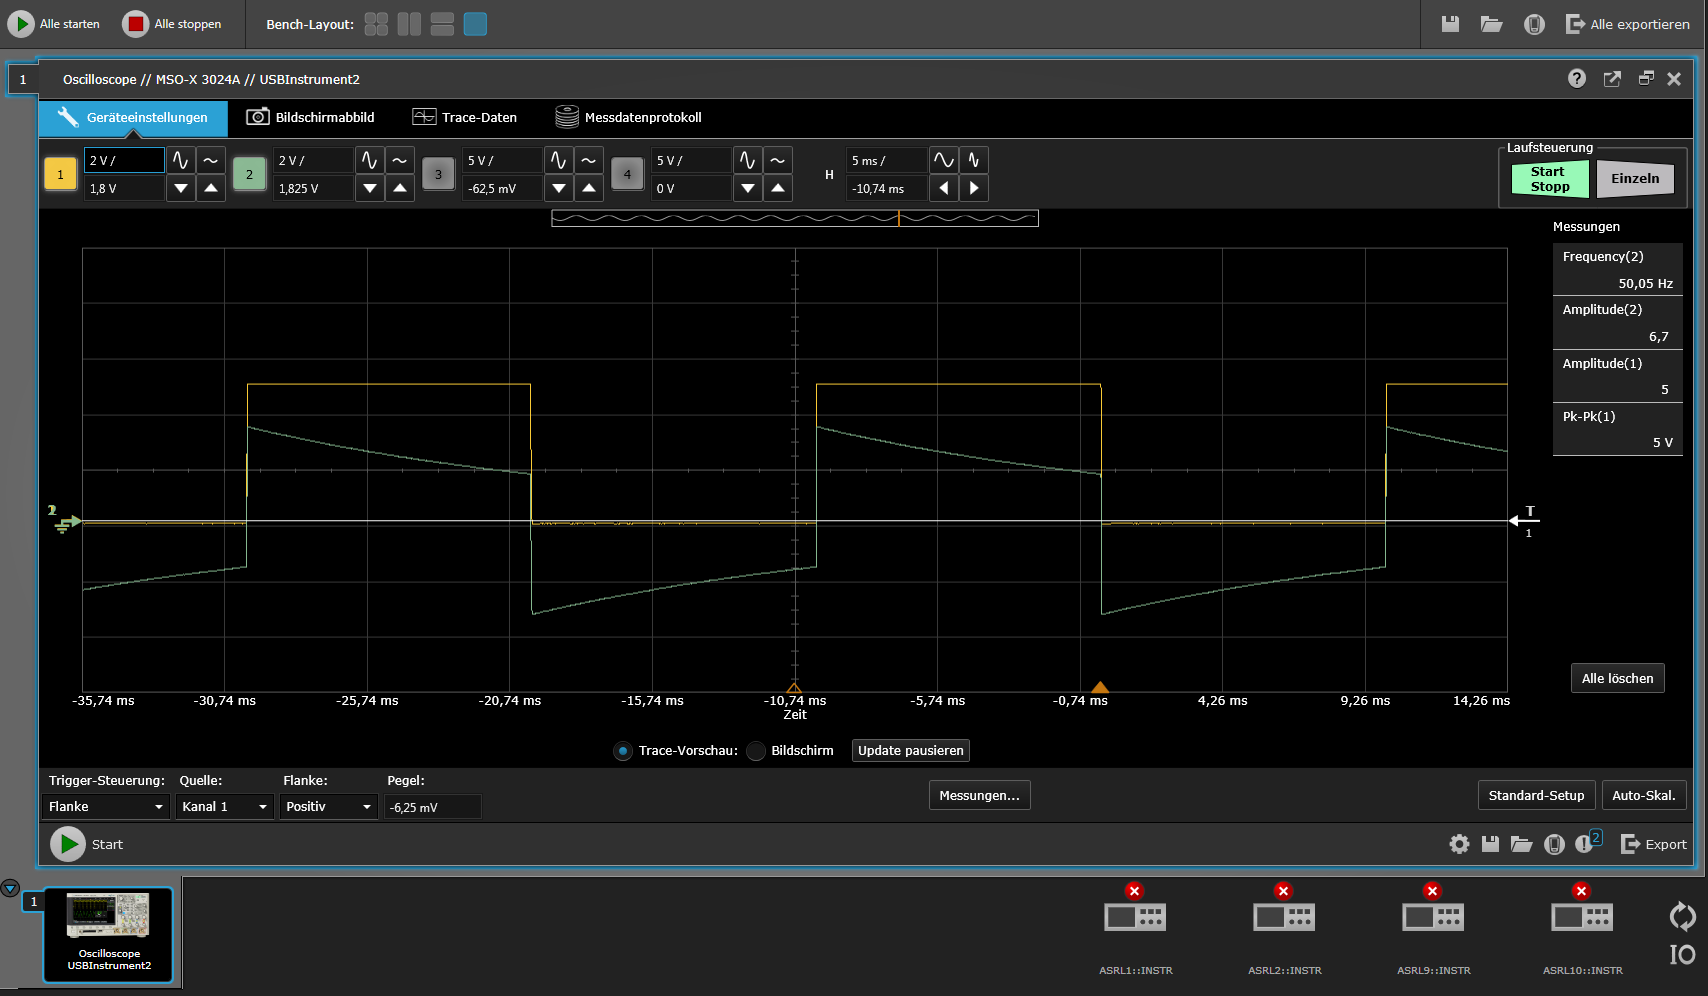
\includegraphics[width=0.6\textwidth]{includes/kom/graphics/MessungWindel_1Ohm_2_2u}
	\caption{Messung mit trockener Windel}
	\label{fig:cap_sensor_dry}
\end{figure}

Wie zu beobachten nimmt die Spannung zwischen den beiden Leiterbahnen der trockenen Windel während eines Rechteckszyklus nur gering ab, die Kapazität bleibt nahezu konstant.

\begin{figure}[ht]
	\centering
		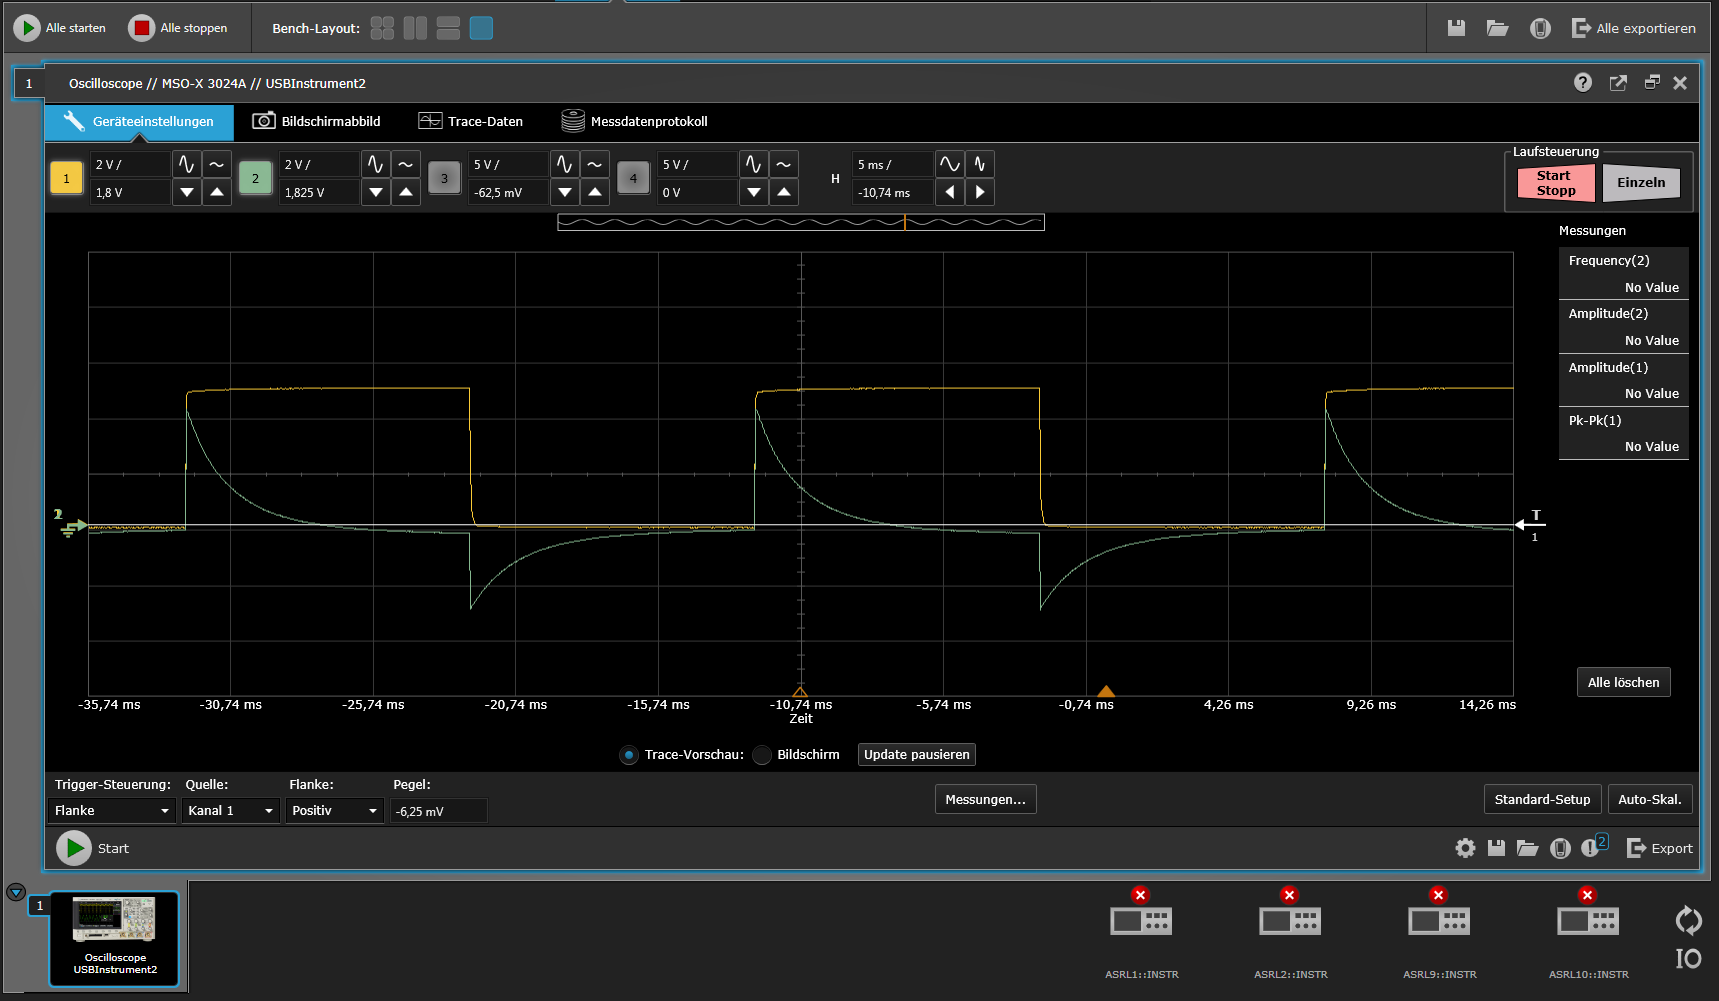
\includegraphics[width=0.6\textwidth]{includes/kom/graphics/MessungWindelnass_1Ohm_2_2u}
	\caption{Messung mit nasser Windel}
	\label{fig:cap_sensor_wet}
\end{figure}

Das Problem mit dem nicht isolierten (siehe Kapitel "Probleme") ist der enstehende Stromfluss, die Leiterbahnen sind leitend miteinander verbunden.

\subsubsection{Probleme}
Beim Sensoraufbau stellten sich zwei große Probleme mit den vorhandenen Metallfäden heraus.

Einerseits lassen sich die Metallfäden nicht an andere Kabel löten, da das Metallgarn meist eine Beschichtung aus Aluminium\footnote{http://www.patent-de.com/20070531/DE60305694T2.html} hat. Dieser Umstand machte das Testen und den Versuchsaufbau umständlich und instabil.

Andererseits war das Metallgarn durch seine Beschichtung nicht vollständing elektrisch isoliert. Ist die Windel mit dem eingenähten Garn nun nass geworden waren die zwei Fäden nicht mehr isoliert zu einandander und der aufgebaute Kondensator verlor seine Kapazität. 

\subsection{Fazit}
Mit dem jetzigen Stand kann man verlässlich die Feuchtigkeit in der Windel detektieren. Dazu wird nicht nur die Feuchtigkeit sondern auch ein rabiater Temperaturanstieg gemessen. Zeigen beide Sensoren eine große Veränderung kann man davon ausgehen das Baby soweit in die Windel uriniert hat. 
Eines der größeren Probleme ist mit Sicherheit das Metallgarn. Hier lässt sich der Sensor optimieren indem man einen vollständig elektrisch isolierten Leiter findet. Ebenfalls lässt sich die Verarbeitungsmöglichkeit des Metallgarns noch verbessern oder geeignete Löt- oder Klebeverfahren finden.

Nichtsdestrotz machen die Sensoren genau das was wir uns am Anfang des Projekts als Ziel gesetzt haben. Die Sensoren detektieren Feuchtigkeit und Wärmeanstieg verlässlich und lassen sich in die Windel integrieren. 

\pagebreak